\section{Generative Knowledge Graph Anomaly Correction}
\label{sec: kg_generation}

In this chapter so far, we have seen techniques for solving scalability issues of generative models for graphs with impressive outcomes. However, none of the data came from domains where knowledge graphs have the most application. In fact, knowledge graph research that considers generative experiments is extremely rare, but this is to be expected. A knowledge base is intended to be a comprehensive collection of relational data that has been curated through a well-designed and controlled schema-based deterministic process, with the goal of representing axiomatic facts from which new, emergent information is inferred through likelihood-estimation-like tasks. There is thus never a need to model a distribution of possible small knowledge graphs that arises from some inherent stochasticity of this process or from nature. But to be specific, this was the case before knowledge graph sizes reached Big Data levels, causing data errors to propagate too far, and stochastic models and algorithms began to be employed for their construction. 

As such, before closing off this thesis work, we present our proposal for generative knowledge graph correction in this section, as a pure application of clever dataset construction techniques and distribution learning with well-renowned graph generative models. The approach detailed here should serve as a promising proof of concept for further development. 

\subsection{The Need to Correct Knowledge with Diffusion}

Recall that knowledge graphs represent structured real-world information modeled as a set of triplets
of head entity, relation, and tail entity. Many modern graphs are constructed automatically from
text or manually curated classically. Regardless of the construction method, massive knowledge graphs often suffer from misinformation, incompleteness, and general noise, which hinder their reliability and utility. These issues began cropping up in recent years, in part, due to the increasing heterogeneity and bulk of data sources that are used to construct the database, where schema mismatches cause nodes and edges to be connected to incorrect subgraphs, often with incorrect labels, as well as data being lost during migration. However, these issues in other or the same cases can arise from the use of artificial intelligence in parsing text documents to attempt to extract all new facts from them. It is evident that these kinds of defects in knowledge graph data that will be used to train a query answering model could cause serious damage.

This noise, during knowledge graph representation, will be expressed through the presence of spurious false-positive triplets, which should be corrected or removed, and the absence of many triplets that are facts but have been labeled as false negatives. From this point onwards, in order to formalize the problem statement and potential solutions, we will assume that we are already in possession of link prediction and query answering models trained on clean data, but several newly modified $n \times n$ blocks of the immense adjacency matrix have been flagged as potentially noisy, thus we have to propose a denoising algorithm to immediately repair them (while assuming the blocks are small enough such that localized modifications will not propagate to the full graph).

Since we are in the possession of powerful knowledge graph reasoning models envisioned as almost perfect oracles for \emph{detecting} anomalies, let's propose a first naive algorithm for knowledge graph anomaly \emph{correction} as an application of these models and what we have seen in Chapter \ref{chp: kg_reasoning}:

\begin{enumerate}
    \item For each adjacency block, perform link prediction over the whole block to estimate the likelihood of false positives and false negatives. If all edge entries are deemed likely, stop the execution. If not, continue to step 2.
    \item For each erroneous entry, perform query answering to propose an alternative edge or suggest removal. Apply the necessary edge flips and continue to step 3.
    \item Since this data is now assumed to be ready for training, update the link prediction and query answering models with an optimization algorithm until convergence for these blocks. But the models are now different, so go back to step 1 to re-evaluate the noise probabilities.
\end{enumerate}

It is very easy to deduce the huge computational cost of this approach, even with one candidate noisy block. If $\abs{V}$ is the total number of nodes in the knowledge graph, $n < \emph{V}$ is the number of nodes in each block, $m$ is the number of negative samples to compute the contrastive loss (\ref{eq:contrastive_loss}), and $n_e$ is the maximum number of training epochs required, from knowledge graph representation theory we know the worst case complexity of each of the three steps is: $O\of{n^2}$, $O\of{n^2|V|}$ and $O\of{n^2 \of{m+1}n_e}$, respectively. However, the biggest issue is the outer loop cost, where in the worst case, in each iteration of the three steps, the likelihood of only one adjacency entry flipped, and the algorithm looped $O\of{n^2}$ times. Altogether, this would amount to $O\of{n^4\of{1+|V|+\of{m+1}n_e}}$ cost. 

The cause of the high-degree polynomial computational complexity of this \emph{exact} knowledge graph anomaly correction algorithm is the model's lack of likelihood estimation power \emph{beyond the range of a single edge} and the lack of \emph{intrinsic estimates of the noise level} in the data. Without these properties, for this difficult application, simple transductive classification models have to behave exactly like the deterministic algorithms they emulate.

On the other hand, imagine if a graph generative model had been trained on a dataset of known clean $n \times n$ graph blocks, where artificial noise was added during training in order to instill denoising behaviour, then applied to perform the anomaly correction on our noisy set as evaluation. Specifically, diffusion models would be the most powerful, due to possessing one denoising model for each noise level in a large range. We will obtain in just $O(n^2 T)$ steps a candidate corrected graph from a wide range of possible noisy inputs, although the output will be stochastic and effectively an approximation of the true \emph{optimal} graph. These kinds of experiments are exactly what this penultimate section of this work will describe.

\subsection{Related work}

Previous literature on knowledge graph subgraph generation is expectedly sparse, and the few works are very recent, which signals a fairly contemporary nature of the problem and its difficulty. 

\cite{thanapalasingam_intelligraphs_2023} is one of the first works on the topic, which unfortunately yielded an approach lacking success. Nevertheless, the authors contribute a dataset of interesting knowledge subgraphs for benchmarking, although we chose to sample our own datasets from the classical academic knowledge graphs.

\cite{mahmoudzadeh_deep_2024} proposes Variational Auto-Encoder (VAE) models for the task, but the approach is still only used to answer queries generatively and not to estimate the graph distribution. We also believe the state-of-the-art performance of diffusion models for graphs motivates the higher relevance of the investigation of the application of these models, as well as their natural compatibility with the problem. 

A very interesting recent approach is detailed in \cite{dong_refining_2025}, where the next-token prediction power of Large Language Models (LLMs) was applied to estimate noise in collections of candidate triplets by assuming their concatenations of entities and relations are fragments of a bigger story, whose internal consistency the model should classify. We support the soundness of the approach; however, generalization is an issue, as not infrequently entity and relation labels in knowledge graphs are partly symbolic keys, and inferring the story immediately is difficult, so the most general approach should also perform graph structure modelling as well.

\subsection{Experiment setup}

The description of the data sampling and model design of the experiments we performed to demonstrate knowledge graph anomaly correction with diffusion models completely details this work's contributions.

\subsubsection{Data}

Given a large knowledge graph $G=\of{V, E_R, R, \mathbf{X}}$ and $n<|V|$, from it we sample a dataset $\mathcal{D}=\offf{\of{\mathbf{x}_i,A_i,\mathbf{v}_i}}_{i=1}^{N}$ of $n \times n$ dense representations of subgraphs from it to use as candidate noisy blocks, by first assigning a subgraph ID to each node. 

$\mathbf{x}_i \in \mathbb{R}^{n \times F}$ (or $\mathbb{R}^{2n \times F}$ when the subgraph is bipartite) are the node features, $A_i \in \offf{0,1,\dots,|R|}^{n \times n}$ are the relation-labeled adjacencies, and $\mathbf{v}_i \in V^{n}$ (or $V^{2n}$ when the subgraph is bipartite) are the knowledge graph entities which are part of the subgraph.

Due to the node permutation group symmetry of graphs \cite{bronstein_geometric_2021}, the entity-to-subgraph assignment cannot be performed with a default entity ID permutation, and to preserve edge locality within subgraphs, we chose to employ depth-first-search-based topological sorting and subgraph splitting based on cutting DFS spanning tree branches. The full dataset construction procedure is detailed in Algorithm \ref{alg:knowledge_correction_dataset}. Note that for computational feasibility and relevance, we only consider sufficiently dense adjacency blocks as valid samples (arbitrarily, we chose the cutoff of 5 edges). 

\begin{algorithm}[hb!]%[H]
    \caption{Knowledge correction dataset sampling}
    \label{alg:knowledge_correction_dataset}
    \begin{algorithmic}
        \STATE{\textbf{input}: knowledge graph $G=\of{V, E_R, R, \mathbf{X}}$, maximal subgraph size $n<|V|$}
        \STATE{$\of{k, l} \gets \of{1, 0}$}
        \STATE{$s:V \to \mathbb{N} \gets$ Map$\of{}$}
        \FOR{$v \in V$}
        \IF{$s\of{v}$ does not exist}
        \STATE{$S\gets\text{Stack}\of{}$}
        \STATE{$\text{StackPush}\of{S,v}$}
        \WHILE{$S$ not empty}
        \STATE{$u\gets\text{StackPop}\of{S}$}
        \IF{$s\of{u}$ does not exist}
        \STATE{$s\of{u}\gets k$}
        \STATE{$l \gets l+1$}
        \IF{$l=n$}
        \STATE{$\of{k,l}\gets \of{k+1,0}$}
        \ENDIF
        \FOR{$w \in N(u)$}
        \STATE{$\text{StackPush}\of{S,w}$}
        \ENDFOR
        \ENDIF
        \ENDWHILE
        \STATE{$\of{k,l}\gets \of{k+1,0}$}
        \ENDIF
        \ENDFOR
        \FOR{$i \gets 1$ to $k-1$}
        \FOR{$j \gets 1$ to $k-1$}
        \STATE{$E_{i,j}\gets\offf{\of{h,r,t} \in E_R \mid s\of{h}=i,s\of{t}=j}$}
        \IF{$\abs{E_{i,j}} \geq 5$}
        \STATE{$\mathbf{v}\gets\offf{u\in V \mid s\of{u} \in \offf{i,j}}$}
        \STATE{$\mathbf{x}\gets\off{\mathbf{X}_u}_{u \in \mathbf{v}}$}
        \STATE{$A\gets\text{ToDense}\of{E_{i,j}}$}
        \STATE{\textbf{yield} $\of{\mathbf{x},A,\mathbf{v}}$}
        \ENDIF
        \ENDFOR
        \ENDFOR
    \end{algorithmic}
\end{algorithm}

As base knowledge graphs to sample from, for this task, we again choose the three classical knowledge graphs which were also evaluating COINs: FB15k-237 \cite{toutanova_observed_2015}, WN18RR \cite{dettmers_convolutional_2018}, and NELL-995 \cite{xiong_deeppath_2017}. The $n \times n$ block datasets sampled from each graph were train-val-test split uniformly at random. For Wordnet, we set $n=10$, while $n=20$ for the other two graphs.

\subsubsection{Model}
The denoising model we employed to perform the anomaly correct is a modified variant of the state-of-the-art graph diffuser DiGress \cite{vignac_digress_2022}, discussed many times before during this chapter. The required modifications arise due to the need for \emph{conditional} diffusion in our setting, as we will focus on denoising adjacency matrices, dependent on the node features and IDs for each subgraph. 
Namely, first on the likelihood modeling side, for each scorer in $\offf{f_t}_{t=1}^T$:
\begin{equation}
    \mathbb{P}\of{A_{t-1} \mid A_t, \mathbf{x}, \mathbf{v}}=\sigma\of{f_t\of{A_{t-1},A_t,\mathbf{x}, \mathbf{v}}}
\end{equation}
Each generator in $\offf{g_t}_{t=1}^T$ thus is trained to maximize the same likelihood:
\begin{equation}
    g_t=\argmin_g{\mathbb{E}_{\mathcal{D},Z_A}\off{-\log\of{\mathbb{P}\of{A_{t-1} \mid A_t, \mathbf{x}, \mathbf{v}}}}},
\end{equation}
where, now internally the graph transformer models of \cite{dwivedi_generalization_2021} employed by the generators possess a knowledge graph entity embedding model $g_V:V\to\mathbb{R}^F$ used to embed the novel input $\mathbf{v}$. 

The entity embeddings are a new hidden state passed through the whole graph transformer, enhancing especially the representation that the FiLM \cite{perez_film_2018} graph attention layers learn.

As a simpler auxiliary knowledge correction task, we also explore \emph{context-based} generation, where, by applying masking during the noising process, only the lower right region of the adjacency samples is denoised, while the remaining three quadrants always remain fixed, serving thus as additional conditioning to help guide more accurate corrections. 

Formally, in this setting:
\begin{align}
    \begin{split}
        A_t &\sim \mathbf{M} \odot \text{Categorical}\of{Q_t \cdot \text{OneHot}\of{A_0}} + \of{1-\mathbf{M}} \odot A_0, \\
        \hat{A}_{t-1} &= \mathbf{M} \odot g_t(\hat{A}_t) + \of{1-\mathbf{M}} \odot A_0, \\
        \forall i,j, \mathbf{M}_{i,j}&=\mathbb{I}\of{i \geq \frac{n}{2}, j \geq \frac{n}{2}}
    \end{split}
\end{align}

\subsubsection{Metrics}

As this section of the work lies in the intersection between knowledge graph reasoning and graph generations, when measuring evaluation performance, we consider both MMD distribution distances to quantify the quality of the learnt subgraph distributions, and edge classification metrics in addition to the contrastive loss for knowledge graphs, in the form for single-hop query answering. Pre-trained TransE \cite{bordes_translating_2013} reasoning models were used to estimate the knowledge graph validity metrics.

\subsection{Results}

Table \ref{tab:kg_diffusion_metrics} presents our numerical results from each experiment.

\begin{table}[H]
    \centering
    \caption{Graph generation and knowledge graph link prediction metrics for the anomaly correction experiments.}
    \label{tab:kg_diffusion_metrics}
    \begin{adjustbox}{width=\textwidth}
    \begin{tabular}{lllrrrrrrrr}
    \toprule
         Dataset & Masked & Split & Degree & Cluster & Orbit & Spectral & Acc. & Pr. & Rec. & F1  \\
    \midrule
         \multirow{4}{*}{FB15k-237} & \multirow{2}{*}{No} & Train & 0.040 & 0.003 & 0.003 & 0.018 & 0.426 & 0.513 & 0.426 & 0.466 \\
         & & Test & 0.244 & 0.001 & 0.001 & 0.010 & 0.071 & 0.094 & 0.071 & 0.081 \\ 
         & \multirow{2}{*}{Yes} & Train & 0.032 & 0.000 & 0.004 & 0.018 & 0.792 & 0.948 & 0.792 & 0.863 \\ 
         & & Test & 0.027 & 0.000 & 0.001 & 0.015 & 0.667 & 0.866 & 0.667 & 0.754 \\ 
         \midrule  
         \multirow{4}{*}{WN18RR} & \multirow{2}{*}{No} & Train & 0.042 & 0.004 & 0.006 & 0.036 & 0.975 & 0.972 & 0.975 & 0.973 \\
         & & Test & 0.051 & 0.166 & 0.043 & 0.039 & 0.032 & 0.027 & 0.032 & 0.029 \\ 
         & \multirow{2}{*}{Yes} & Train & 0.042 & 0.004 & 0.006 & 0.036 & 0.995 & 0.996 & 0.995 & 0.996 \\ 
         & & Test & 0.045 & 0.095 & 0.010 & 0.055 & 0.663 & 0.624 & 0.663 & 0.643 \\ 
         \midrule
         \multirow{4}{*}{NELL-995} & \multirow{2}{*}{No} & Train & 0.068 & 0.001 & 0.060 & 0.043 & 0.555 & 0.581 & 0.555 & 0.567 \\
         & & Test & 0.053 & 0.004 & 0.054 & 0.032 & 0.199 & 0.217 & 0.199 & 0.208 \\ 
         & \multirow{2}{*}{Yes} & Train & 0.061 & 0.000 & 0.074 & 0.050 & 0.904 & 0.966 & 0.904 & 0.934 \\ 
         & & Test & 0.064 & 0.000 & 0.133 & 0.050 & 0.802 & 0.823 & 0.802 & 0.812 \\ 
    \bottomrule
    \end{tabular}
    \end{adjustbox}
\end{table}

First, we observe that the DiGress for KGs had no issues with learning each of the data distributions, with MMDs decently low and comparable to baselines on data from other domains. 

For the fully unmasked experiments, the classification metrics tell a different story. Namely, while for the Wordnet graph, the training distribution seems to have been learned almost perfectly, there is almost no generalization to the test set. On the other hand, for Freebase and NELL, slight underfitting even during training is detected. 

Interestingly, for the masked setting, the results are much more promising, as both sufficient anomaly correction learning and generalization are observed. 

Thus, we hypothesize that, unfortunately, this is due to the difficulty of the problem of correcting fully noisy adjacency matrices such that all triplets are valid facts. To improve model performance, we could employ more bespoke data curation than simple uniform train-test splitting, as well as data augmentation during training, in addition to potentially also designing a bespoke graph transformer architecture for the task of knowledge graph subgraph generation.

Figure \ref{fig:kg_diffusion_loss} provides perhaps the best alternative summary to our experiment results, as well as proving the benefits of employing diffusion models to the task. The plots visualize the distribution of the contrastive loss of the current state of the subgraphs against the number of denoisers applied thus far. 

While achieving the range of TransE loss values of the clean data is often out of reach, during training, the DiGress generators are able to almost monotonically decrease the contrastive loss over time. This is very relevant, as this implies almost all proposed edge flips by DiGress are valid corrections when the model is able to learn and generalize. 

As the examples provided in Figure \ref{fig:kg_diffusion_examples} show, in some cases the quality of the corrected graphs can be extremely high, with very few spurious entity relations.

\begin{figure}[H]
    \centering
    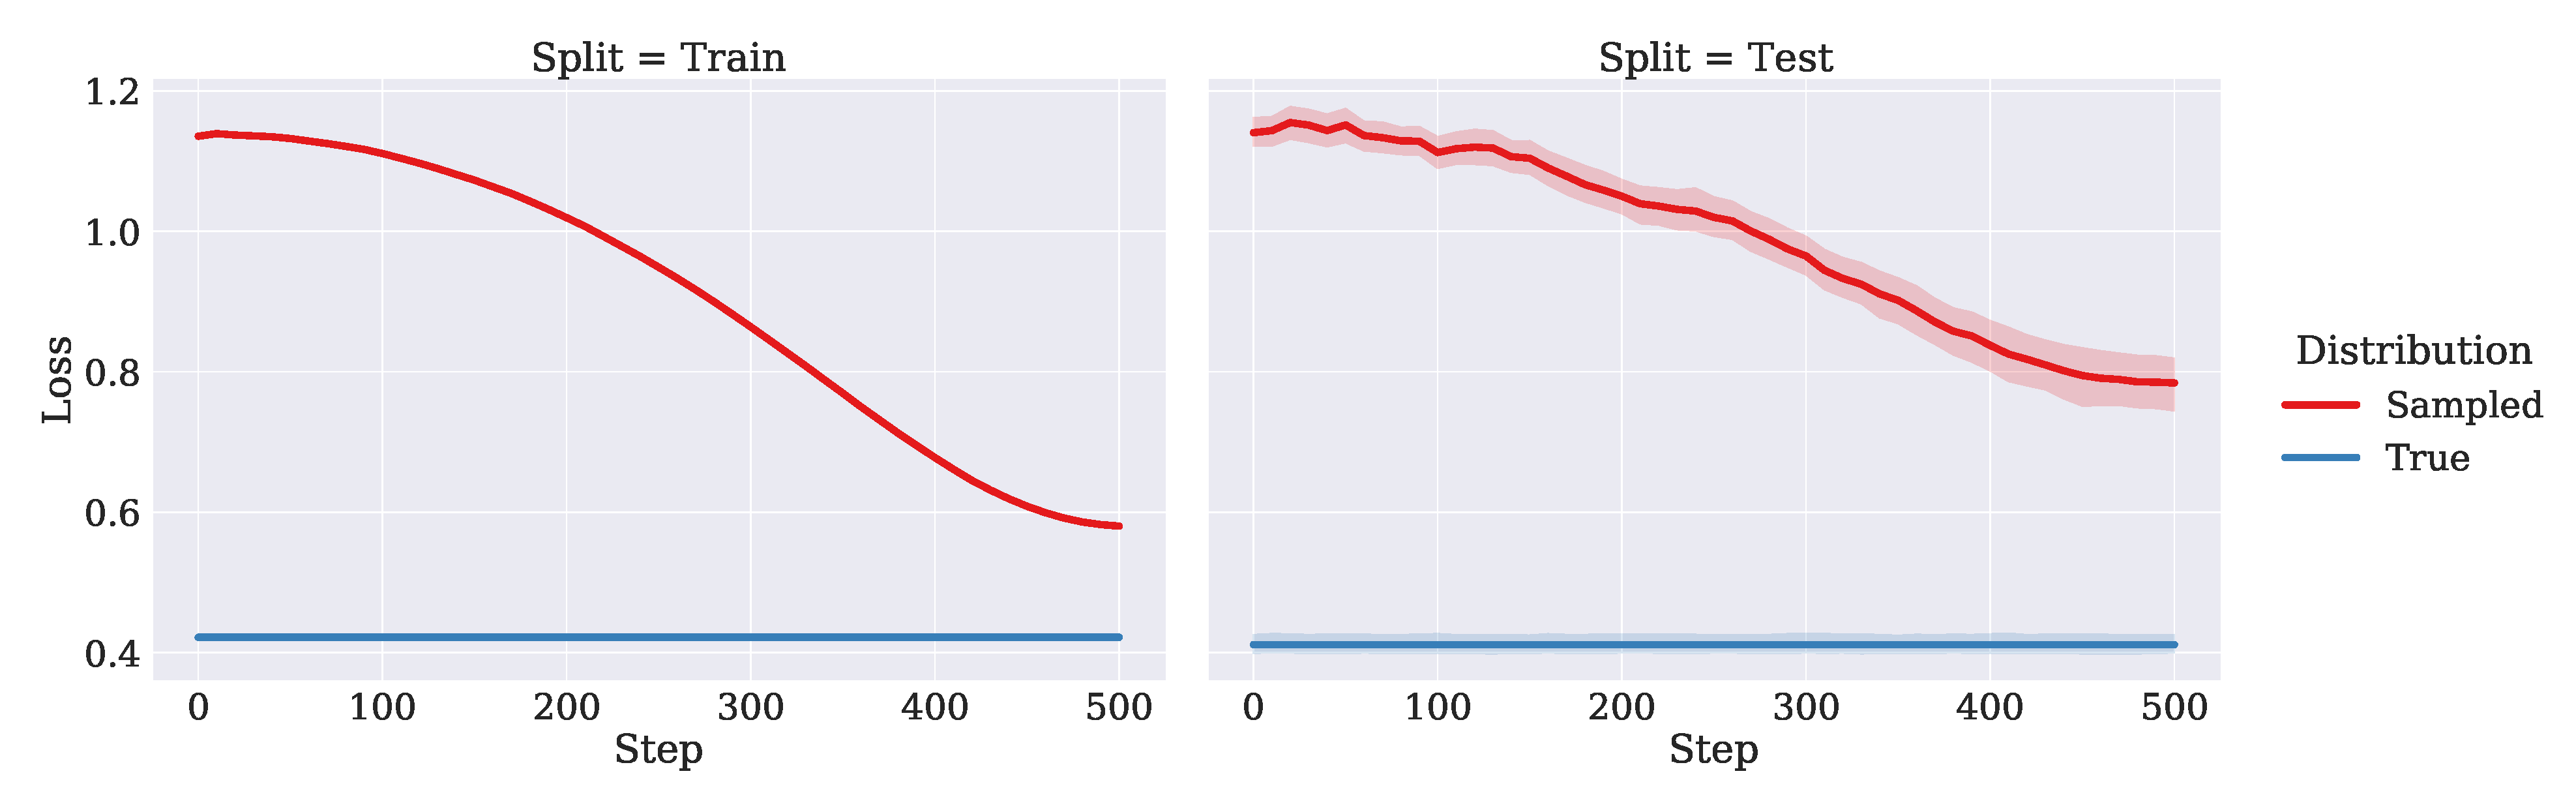
\includegraphics[width=0.49\linewidth]{figures/kg_generation/chain_likelihood_freebase.pdf}
    \hfill
    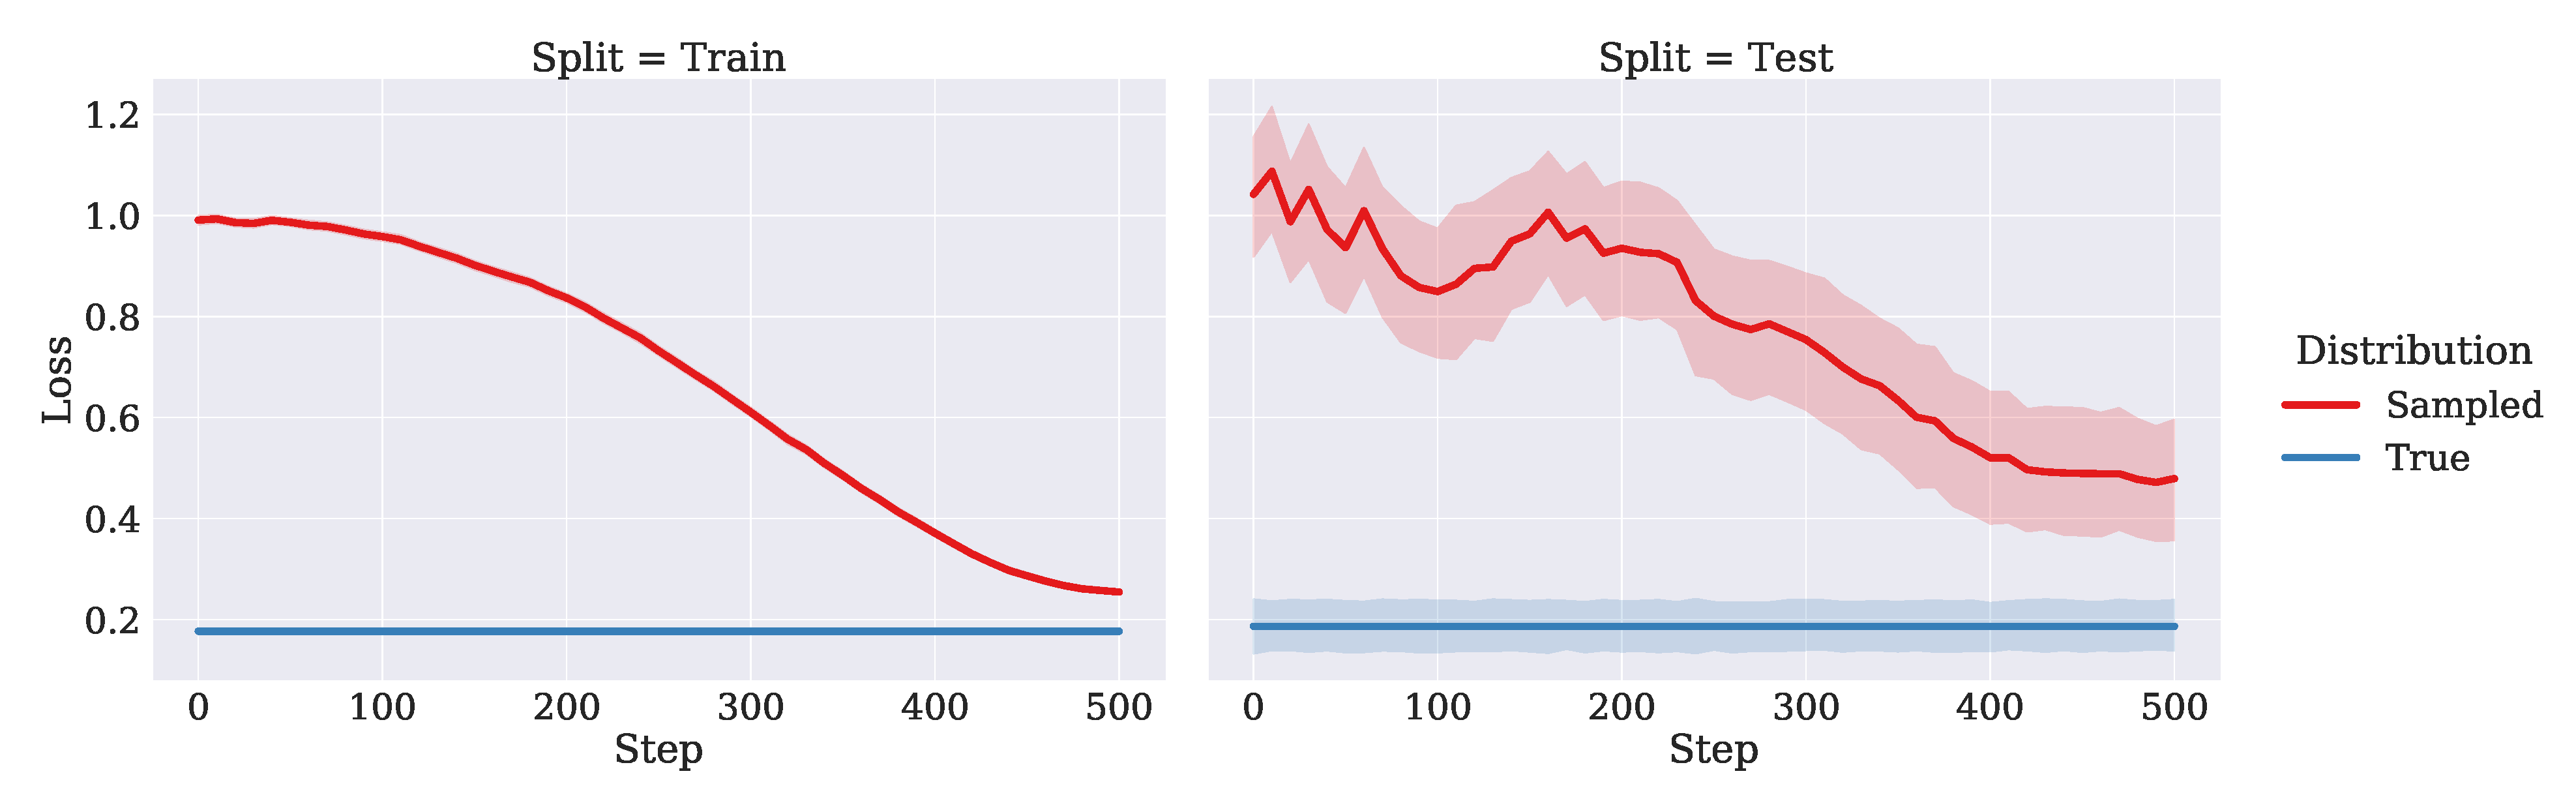
\includegraphics[width=0.49\linewidth]{figures/kg_generation/chain_likelihood_freebase_masked.pdf}
    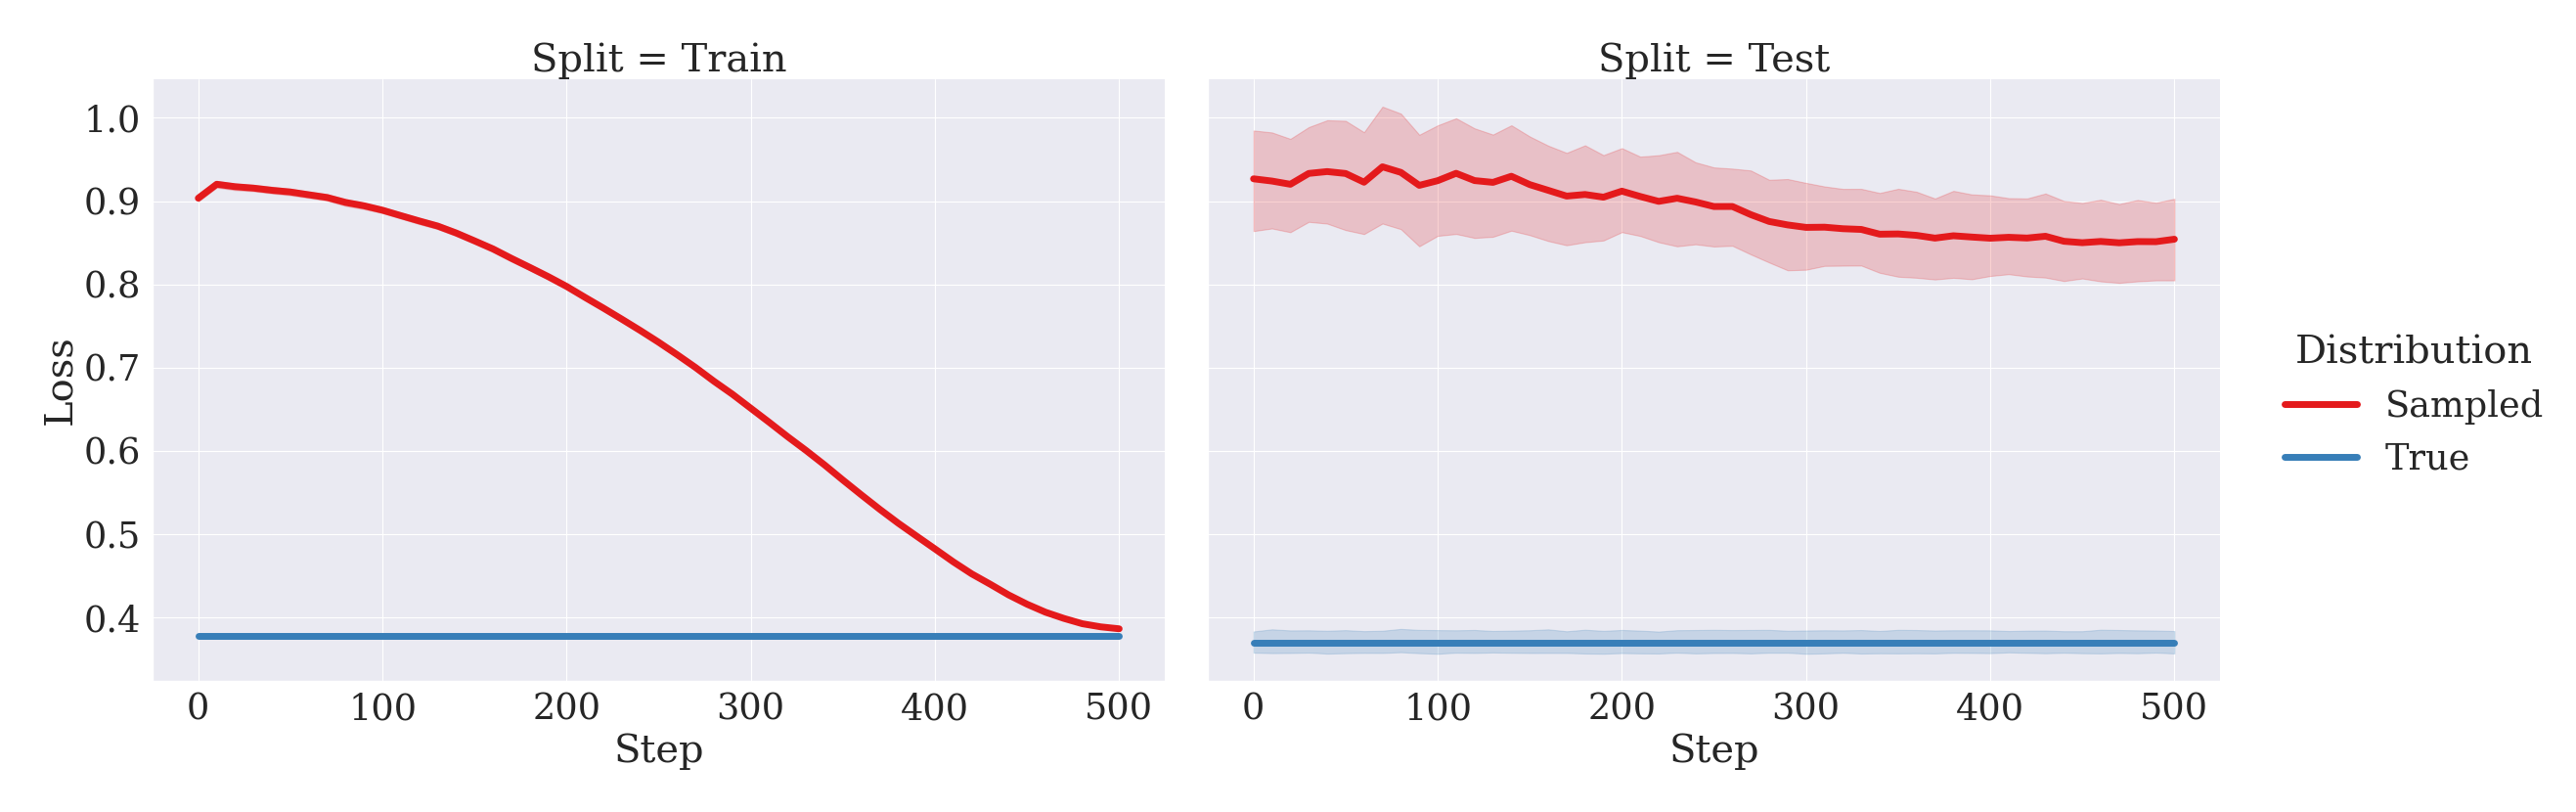
\includegraphics[width=0.49\linewidth]{figures/kg_generation/chain_likelihood_wordnet.png}
    \hfill
    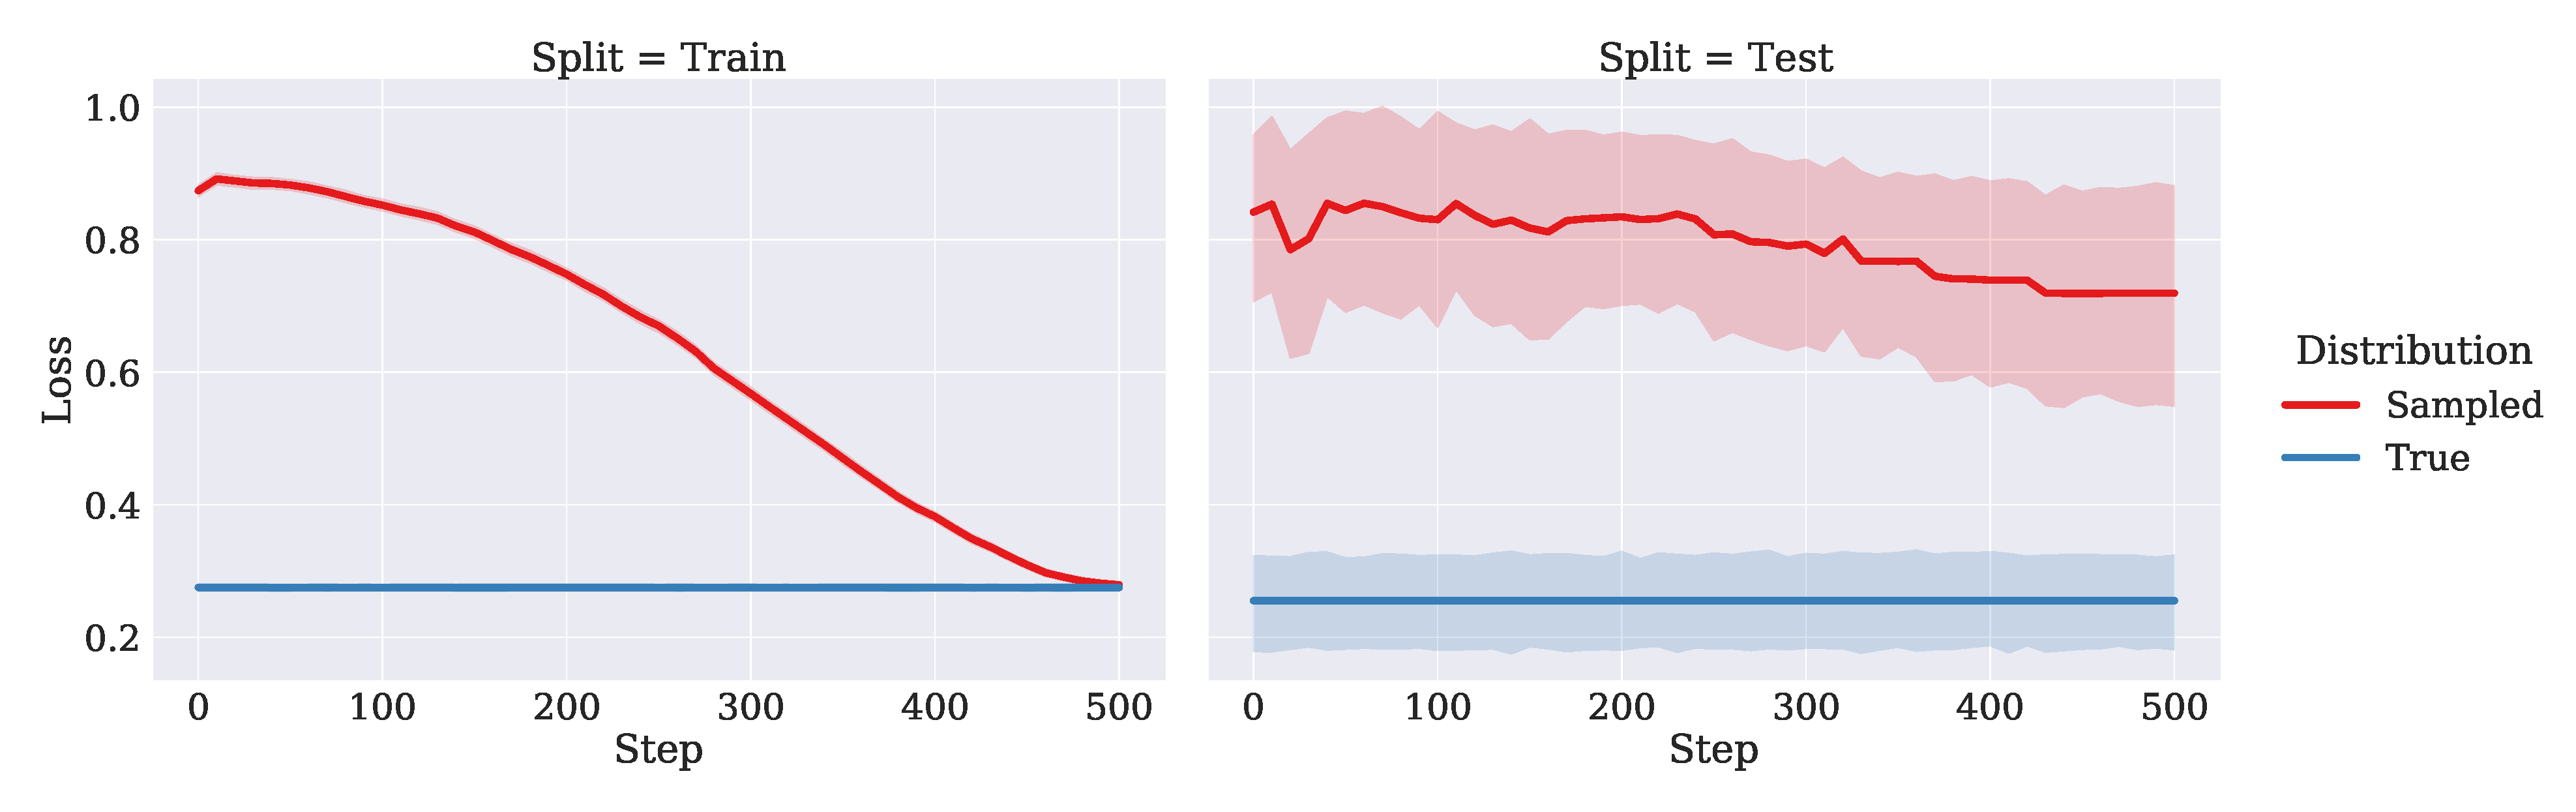
\includegraphics[width=0.49\linewidth]{figures/kg_generation/chain_likelihood_wordnet_masked.pdf}
    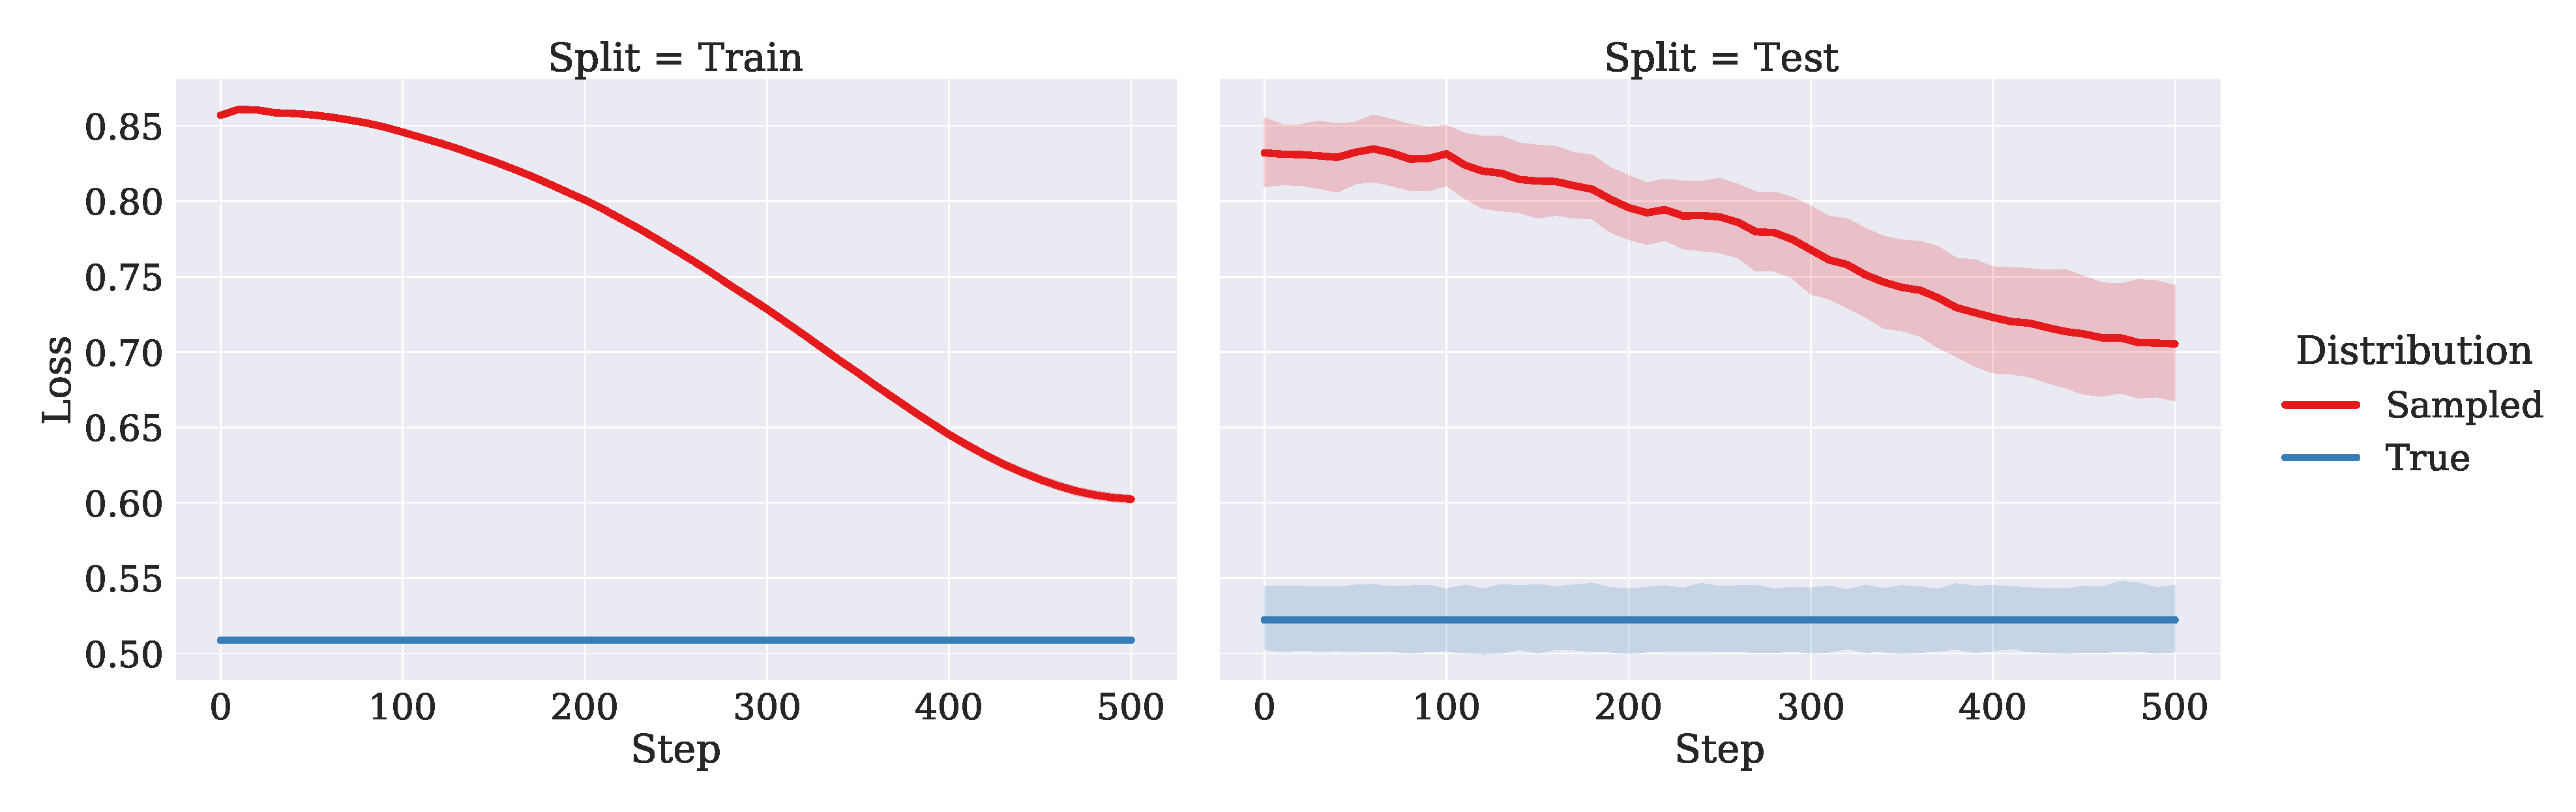
\includegraphics[width=0.49\linewidth]{figures/kg_generation/chain_likelihood_nell.pdf}
    \hfill
    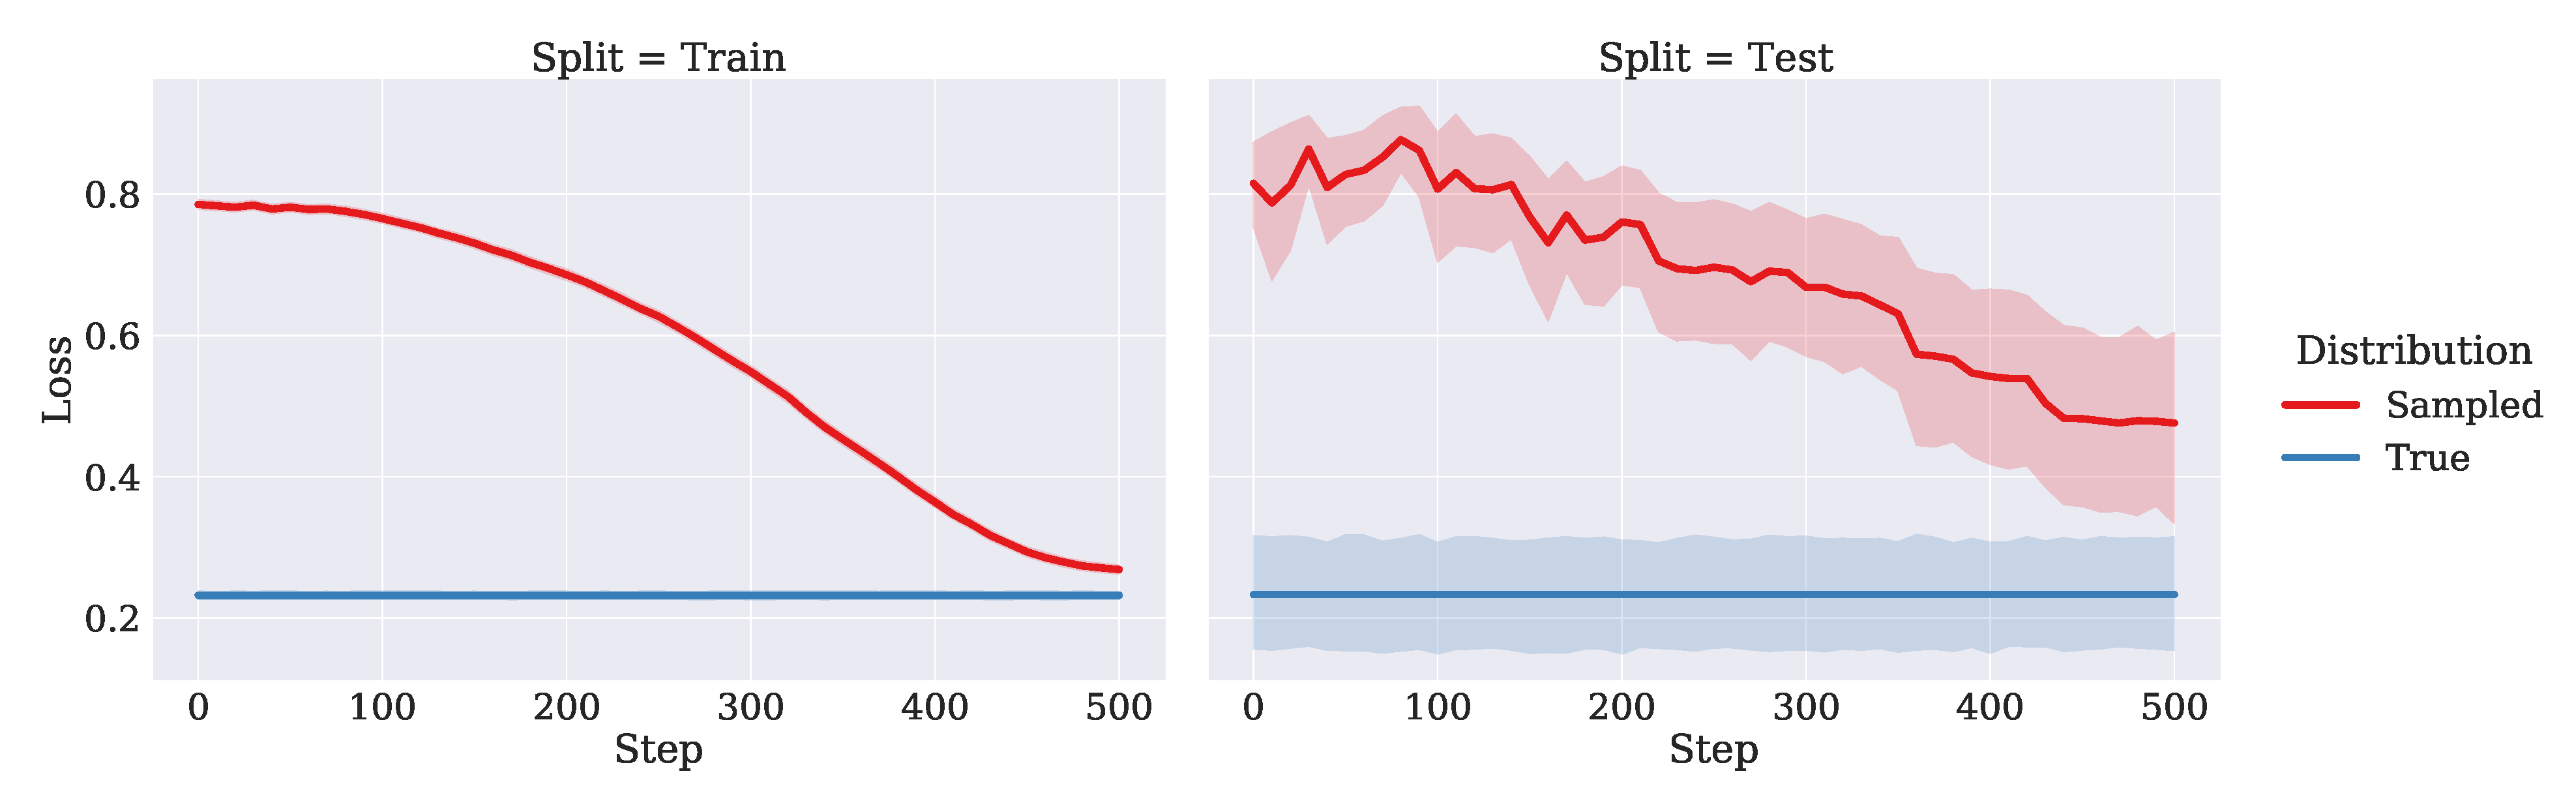
\includegraphics[width=0.49\linewidth]{figures/kg_generation/chain_likelihood_nell_masked.pdf}
    \caption[Knowledge graph contrastive loss across diffusion steps.]{Knowledge graph contrastive loss across diffusion steps. Top to bottom: train vs test splits of different datasets. Left vs right: unmasked vs masked diffusion.}
    \label{fig:kg_diffusion_loss}
\end{figure}

\begin{figure}[H]
    \centering
    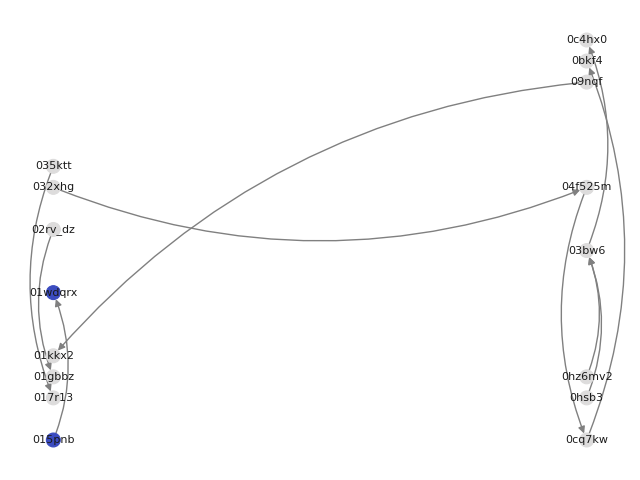
\includegraphics[width=0.16\linewidth]{figures/kg_generation/freebase_noisy.png}
    \hfill
    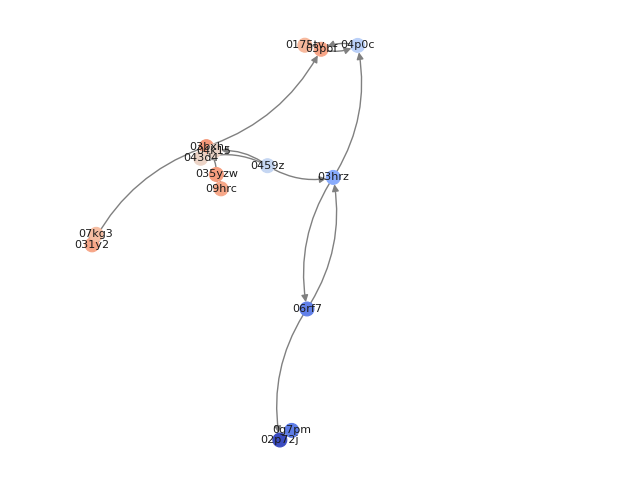
\includegraphics[width=0.16\linewidth]{figures/kg_generation/freebase_masked_noisy.png}
    \hfill
    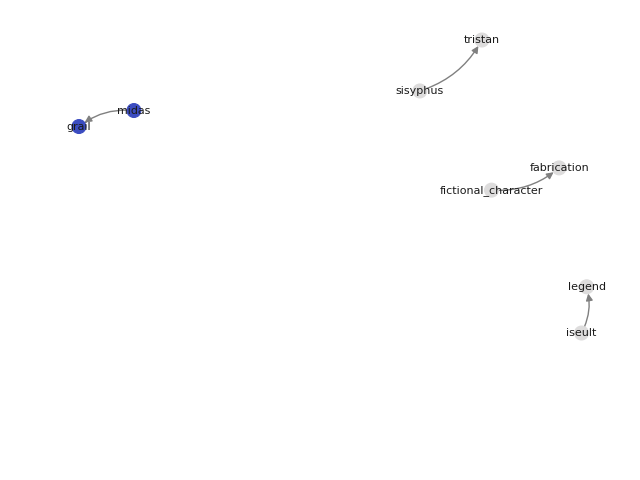
\includegraphics[width=0.16\linewidth]{figures/kg_generation/wordnet_noisy.png}
    \hfill
    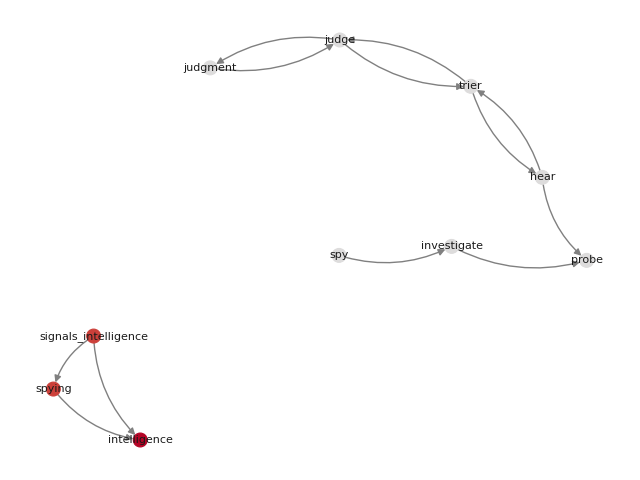
\includegraphics[width=0.16\linewidth]{figures/kg_generation/wordnet_masked_noisy.png}
    \hfill
    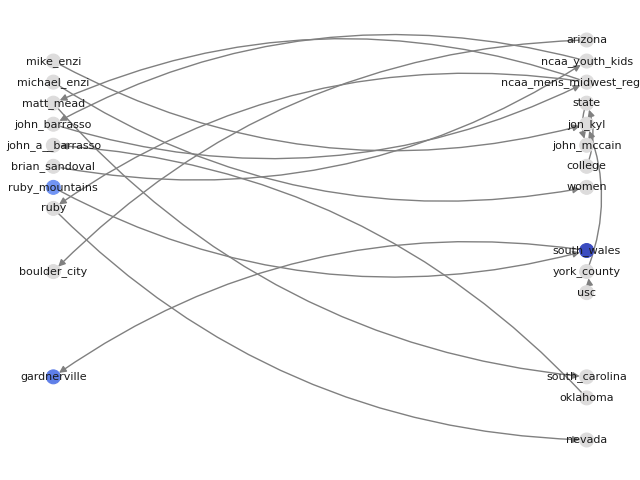
\includegraphics[width=0.16\linewidth]{figures/kg_generation/nell_noisy.png}
    \hfill
    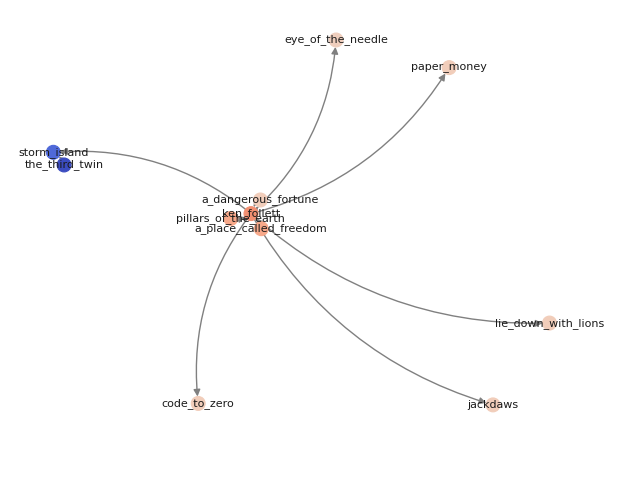
\includegraphics[width=0.16\linewidth]{figures/kg_generation/nell_masked_noisy.png}
    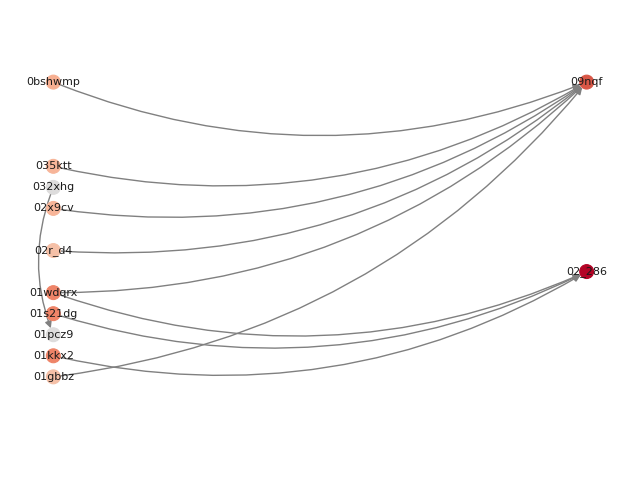
\includegraphics[width=0.16\linewidth]{figures/kg_generation/freebase_clean.png}
    \hfill
    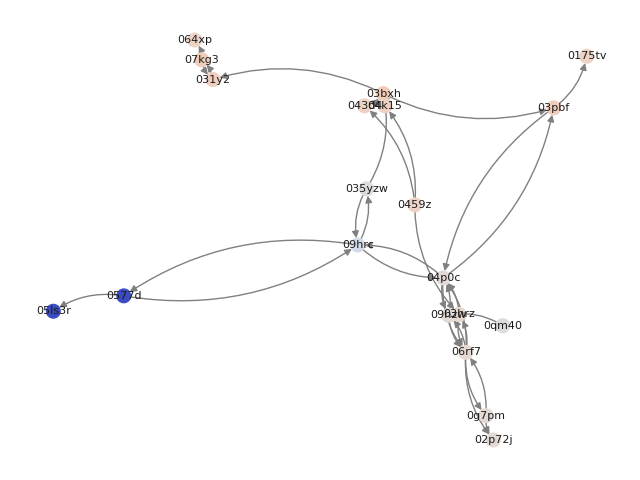
\includegraphics[width=0.16\linewidth]{figures/kg_generation/freebase_masked_clean.png}
    \hfill
    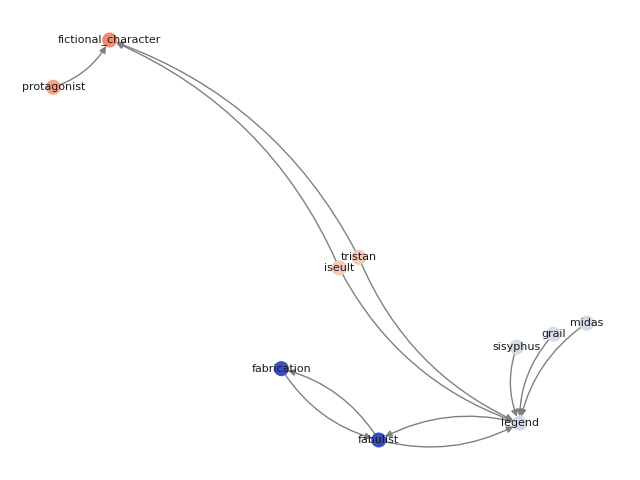
\includegraphics[width=0.16\linewidth]{figures/kg_generation/wordnet_clean.png}
    \hfill
    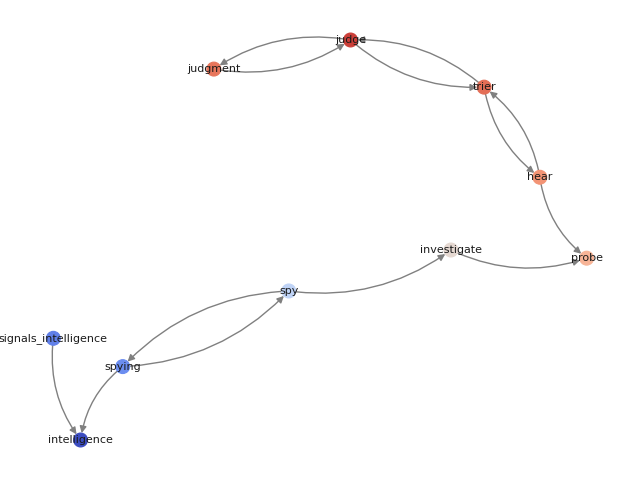
\includegraphics[width=0.16\linewidth]{figures/kg_generation/wordnet_masked_clean.png}
    \hfill
    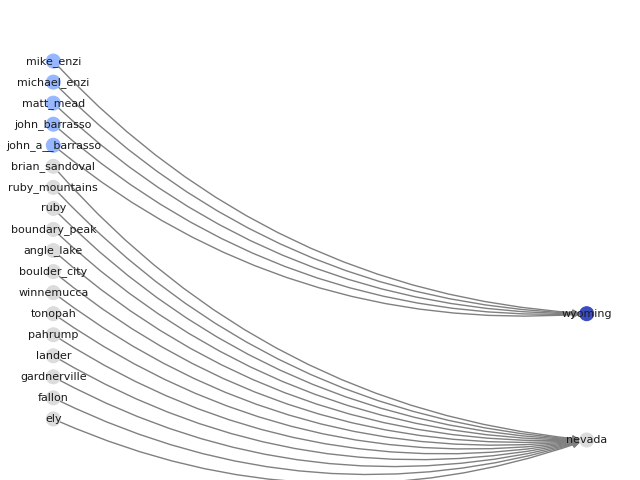
\includegraphics[width=0.16\linewidth]{figures/kg_generation/nell_clean.png}
    \hfill
    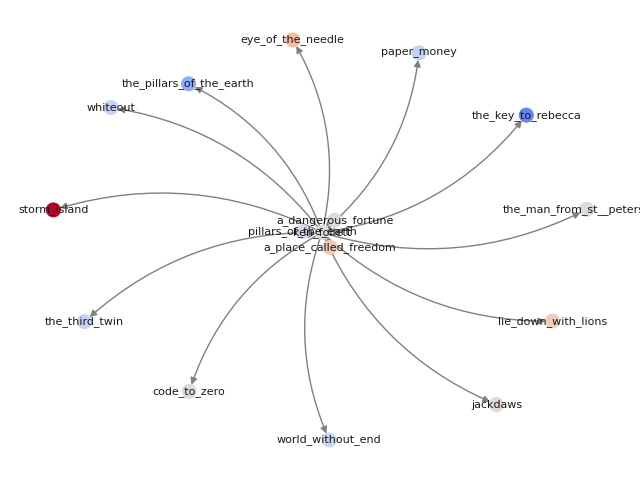
\includegraphics[width=0.16\linewidth]{figures/kg_generation/nell_masked_clean.png}
    \caption[Visual examples of knowledge graph anomaly correction.]{Visual examples of knowledge graph anomaly correction obtained during training. Left to right: unmasked vs masked examples of different datasets. Top vs bottom: noisy input vs denoised output.}
    \label{fig:kg_diffusion_examples}
\end{figure}

\subsection{Summary}
As a way to conclude this enlightening exploration into the application possibilities of generative models to knowledge graphs, we discuss a sort of textual Venn diagram between the content of the last two chapters of this thesis. 

The intersection between knowledge graph reasoning and graph generation models lies in their joint ability to model edge likelihood, and this was enough motivation for us to discuss proposing new knowledge triplets via a diffusion model in this section. Generative graph models have the additional power to sample various other features of graphs, such as node and graph-level attributes, while also internally performing estimates of noise levels in graph data and supporting chaining correlated samples. However, on the other hand, query answering models for knowledge graphs are much more tuned to modeling complex first-order logic over very large graphs, have impressive knowledge pattern detection capabilities, and the possibility of targeted information retrieval through sample ranking.